%!TEX root = SYN.tex

\chapter[State Of The Art]{State Of The Art}
\graphicspath{ {images/stateOfArt} }



\section{Software Visualization}


\begin{wrapfigure}{r}{0.3\textwidth}
  \centering
  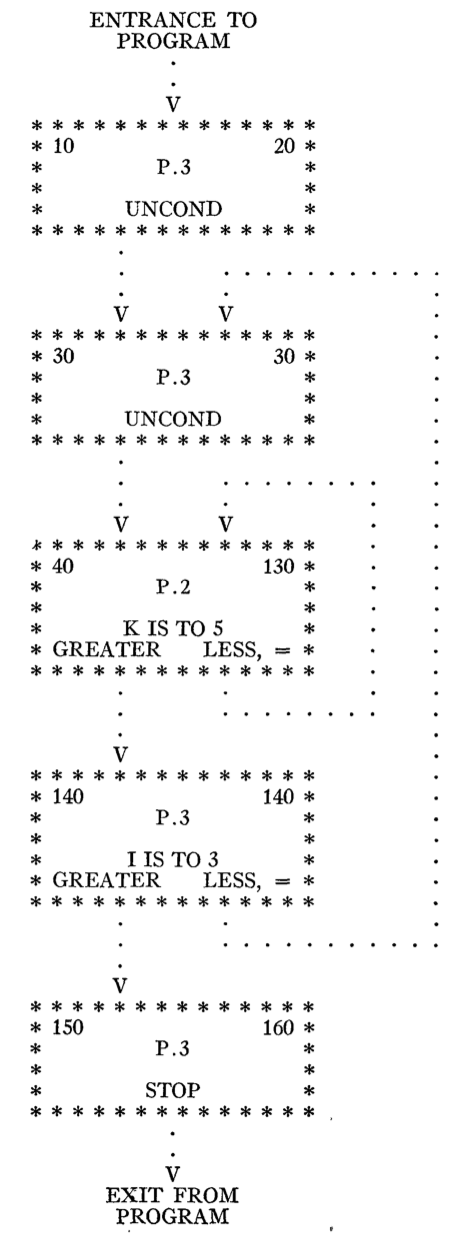
\includegraphics[width=0.9\linewidth]{Haibt1959_Flowchart.png} 
  \caption{Flowchart presented by Haibt in 1959}
  \label{fig:Haibt1959_Flowchart}

\end{wrapfigure}

Software maintenance and evolution are essential parts of the software development lifecycle. Both require that developers deeply understand their system. 
Mayrhauser and Vans defined {\it program comprehension} as a process of \quotes{\textit{knowledge to acquire new knowledge}} \cite{VonMayrhauser1995}. 
Generally, programmers possess two types of knowledge: general and software-specific knowledge. 
Software comprehension aims to increase this specific of the system and can leverage software visualization techniques for this purpose. 
Software visualization supports understanding software systems by visually presenting various information about them, e.g., their architecture, source code, or behavior.
Stasko et al. \cite{Stasko2008} conducted a study in 1998 that shows how visualization arguments human memory since 
it works as external cognitive aid and thus, improves thinking and analysis capabilities.

There are cases when software visualization can be used to aid the analysis activity. For example, when programmers need to comprehend the architecture of a system \cite{Panas2007}, when researchers analyze version control repositories \cite{Greene2017}, or to support developers' activities \cite{LopezHerrejon2018}. 

According to Butler et al. \cite{Butler1993} there are three categories of visualization:
\begin{itemize}
	 \item Descriptive visualization. Widely used for education purposes, the visualization is used to present data to other people. 
	 \item Explorative visualization. Used to discover the nature of the data being analyzed. With this visualization, the users do not necessarily know what they are looking for; e.g. they explore possibilities for improvement.
	 \item Analytical visualization. Adapted when we need to find something known in the available data. 
\end{itemize}
	% Dijkstra1971a
Software visualization approaches vary with respect to two dimensions: the level of abstraction and the visualized data.
According to the type of the data, we can classify visualization as:
\begin{itemize}
	\item Evolutionary visualizations: Depicts the development history of a system. Mainly used to find the cause of problems in software. 
	\item Static visualizations: Used to present information extracted with static analysis of the software. It provides information about the structure of the system.
	\item Dynamic visualizations: Shows results of dynamic instrumentation of the software execution. It provides information about the behavior of the system.
\end{itemize}

Moreover, the level of abstraction can be classified as follows:
\begin{itemize}
	\item Code-level visualization: where fine granted sourcecode information is highlighted, such as the lines of code. 
	\item Design-level visualization: used to visualize self-contained source code entities, such as classes in object-oriented systems. 
	\item Architectural-level visualization: depicts the system architecture and the relationships among its components. 
\end{itemize}


% \subsection*{History of software visualization}

The earliest software visualization techniques in the literature used 2D diagrams. 
For example, Haibt, used them already in 1959 and provided a graphical outline of a program and its behavior with flowcharts \cite{Haibt1959}. 
As shown in \autoref{fig:Haibt1959_Flowchart}, they were 2D diagrams that described the execution of a program.
He wrapped each statement in a box, representing the control flow with arrows.
Ten years later, Knuth confirmed the effectiveness of flowcharts \cite{Knuth1963}. 
He found that programs around that time were affected by a lack of readability.
Therefore, he introduced a tool to generate visualizations from the software documentation automatically.
Nassi and Schneiderman \cite{Nassi1973}, in 1973, introduced the Nassi–Shneiderman diagram (NSD), shown in \autoref{fig:Nassi1973_NSD}, to represent the structure of a program. 
The diagram was divided into multiple sub-blocks, each with a given semantic based on its shape and position. 
In the 80s, researchers followed two main directions for software visualization. The first was the source code presentation.
For example, Hueras and Ledgard \cite{Hueras1977} then Waters \cite{Waters1983} developed techniques to format the source code with a prettyprinter. 
The second direction was the program behavior, mainly for educational purposes.
One of that period's most prominent visualization systems was Balsa-II \cite{Brown1988} (\autoref{fig:BalsaII}).
Balsa-II was a visualization system that, through animations, displayed the execution of an algorithm.
Programmers could customize the view and the control execution of the algorithm to understand them with a modest amount of effort. 
The program was domain-independent, and learners could use it with any algorithm. 
Around the end of the 80s, Müller et al. \cite{Mueller1988} released Rigi (\autoref{fig:Rigi}), a tool to visualize large programs.
It exploited the graph model, augmented with abstraction mechanisms to represent systems components and relationships. 

\begin{figure}[ht]
  \minipage{0.33\textwidth}
  \centering
    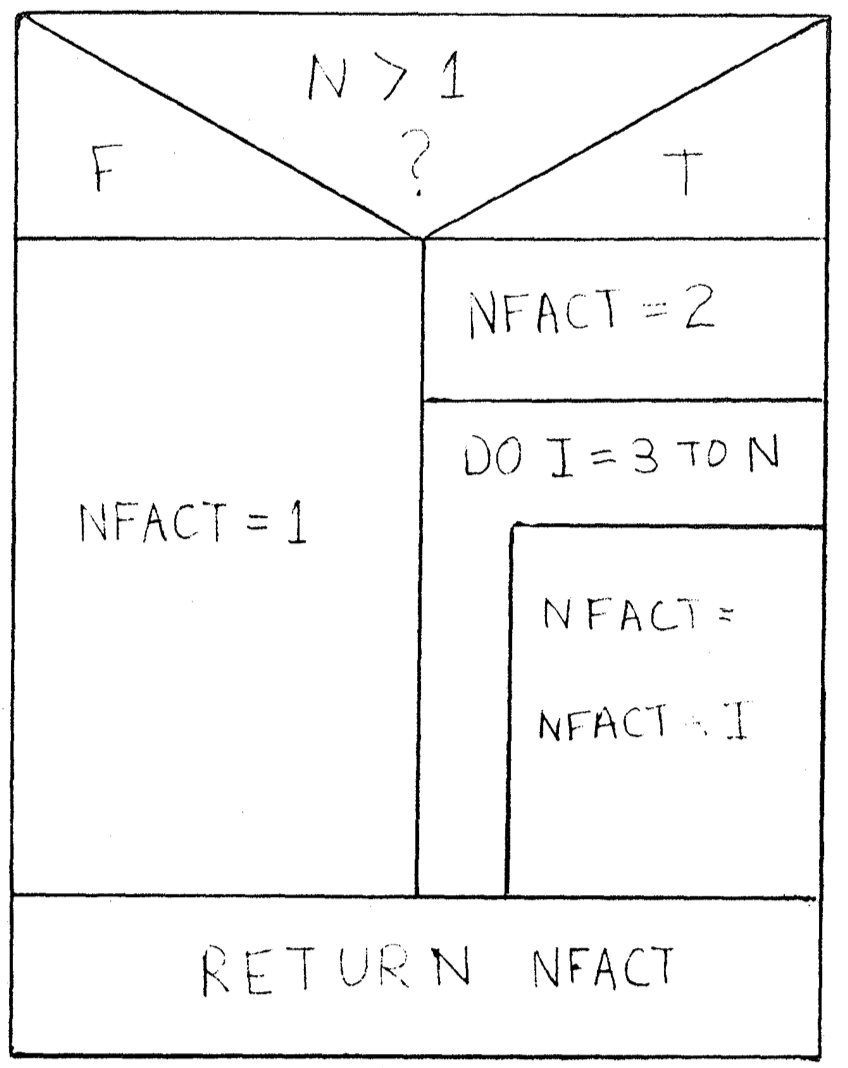
\includegraphics[width=0.8\linewidth]{Nassi1973_NSD.png}
    \caption{NSD of the factorial function.}
    \label{fig:Nassi1973_NSD}
  \endminipage\hfill
  \minipage{0.33\textwidth}
    \centering
    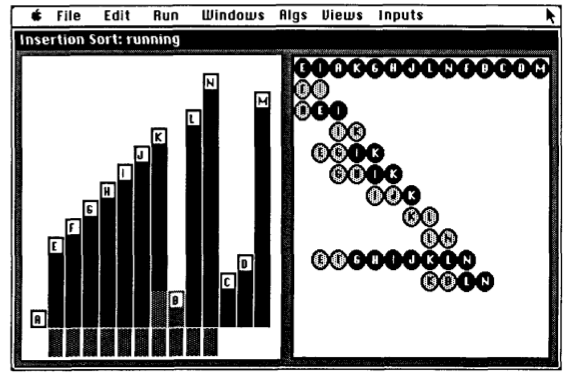
\includegraphics[width=\linewidth]{Brown1988_BalsaII.png}
    \caption{Balsa-II}
    \label{fig:BalsaII}
  \endminipage\hfill
  \minipage{0.33\textwidth}
    \centering
  	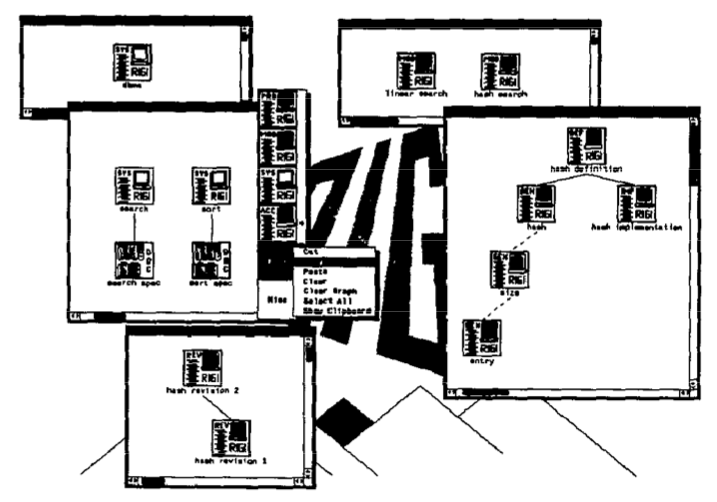
\includegraphics[width=\linewidth]{Mueller1988_Rigi.png}
  	\caption{Rigi}
	\label{fig:Rigi}
\endminipage\hfill
  \end{figure}


  % The growing number of object-oriented programming languages emerging in the mainstream raised 
  % the interest in understanding not only the structure but also the behavior of systems written according to this paradigm. 
  % Kleyn et al. proposed GraphTrace [KG88], a tool using concurrently animated views to visualize dynamic information,
  % Myers's taxonomy of program visualization systems
  % Price et al. proposed a more detailed taxonomy

In the 1990s, there was more interest in the field of software visualization. 
In 1992, Erik et al. introduced a new technique to visualize line-oriented statistics \cite{Eick1992}. 
It was embodied in Seesoft (\autoref{fig:Seesoft}), a software visualization system to analyze and visualize up to 50,000 lines of code simultaneously. 
In their visualization, each line was mapped to a thin row. Each row was associated with a color that described a statistic of interest, e.g., red rows are those most recently changed, and blue are those least recently changed.

One year later, De Pauw et al. \cite{DePauw1993} introduced Jinsight (\autoref{fig:Jinsight}), a tool to provide animated views of object-oriented systems' behavior. 

\begin{figure}[ht]
  \minipage{0.5\textwidth}
  	\centering
    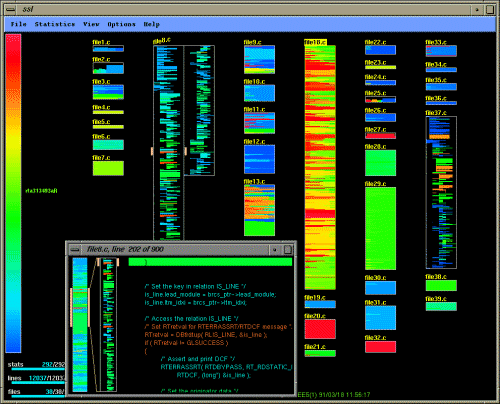
\includegraphics[width=0.8\linewidth]{Eick1992_Seesoft.png}
    \caption{Seesoft}
    \label{fig:Seesoft}
  \endminipage\hfill
  \minipage{0.5\textwidth}
  	\centering
    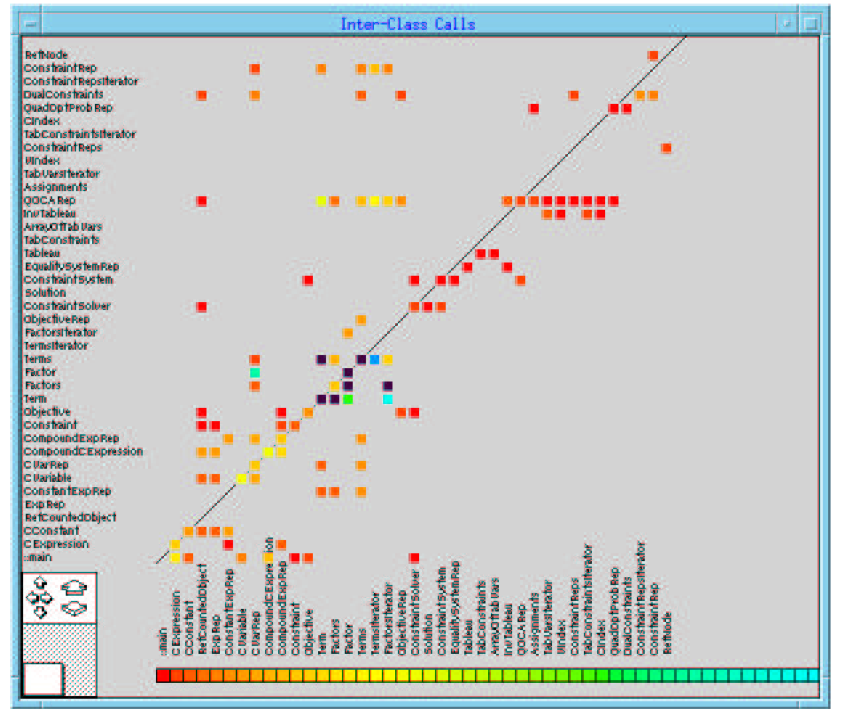
\includegraphics[width=0.8\linewidth]{DePauw1993_Jinsight.png}
    \caption{Jinsight}
    \label{fig:Jinsight}
  \endminipage\hfill
\end{figure}

% the first contributors to software evolution visualization were Holt and Pak in 1996, who used their tool called GASE [HP96]
% 		GASE: visualizing software evolution-in-the-large 

That period was favorable also for experimenting with novel research directions for visualization, 
such as 3D visualization and Virtual Reality. 
% In 1995, Reiss presented a configurable engine for building 3D visualization of programs called PLUM
In 1998, Chuah and Erick \cite{Chuah1998} proposed three techniques to visualize project data. 
They leveraged glyphs, a graphical object that represents data through visual parameters. 
The first technique was the Timewhell glyph (\autoref{fig:Chuan1}), to visualize time-oriented information (number of lines of code, number of errors, number of added lines). 
The second technique was the 3D wheel glyph (\autoref{fig:Chuan2}). It encoded the same attributes of the time wheel and used the height to encode time. 
Infobug (\autoref{fig:Infobug}) glyph was the last technique, where each glyph was composed of four parts, each representing essential data of the system, such as time, code size, and the number of added, deleted, or modified code lines. \newline

\begin{figure}[ht]
\minipage{0.32\textwidth}
\centering
  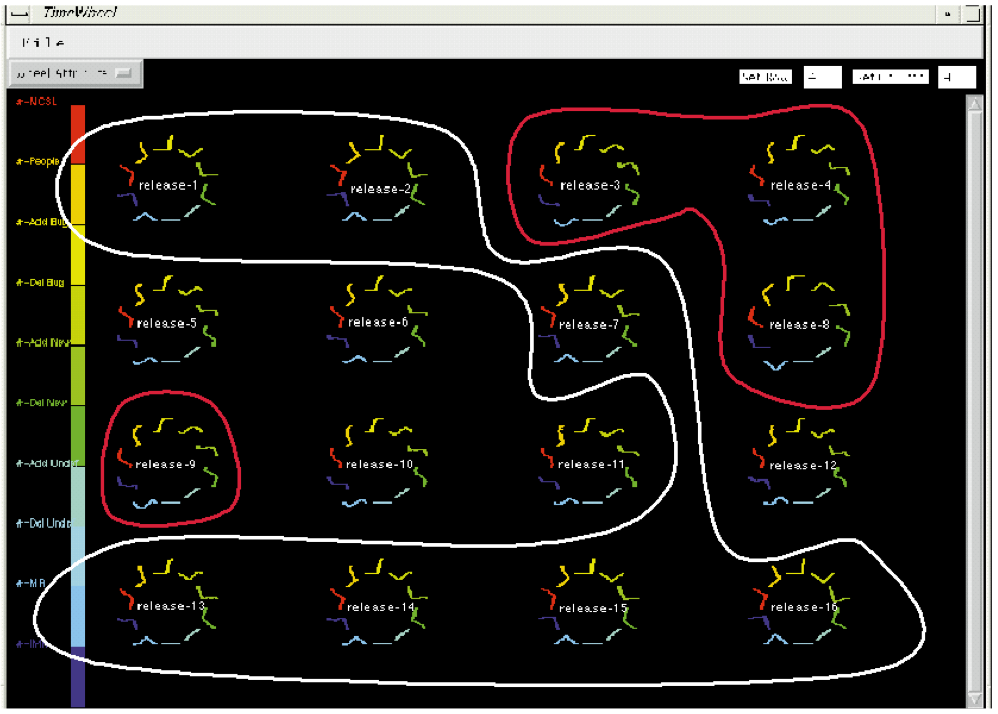
\includegraphics[width=\linewidth]{Chuan1.png}
  \caption{Timewhell}
  \label{fig:Chuan1}
\endminipage\hfill
\minipage{0.32\textwidth}
\centering
  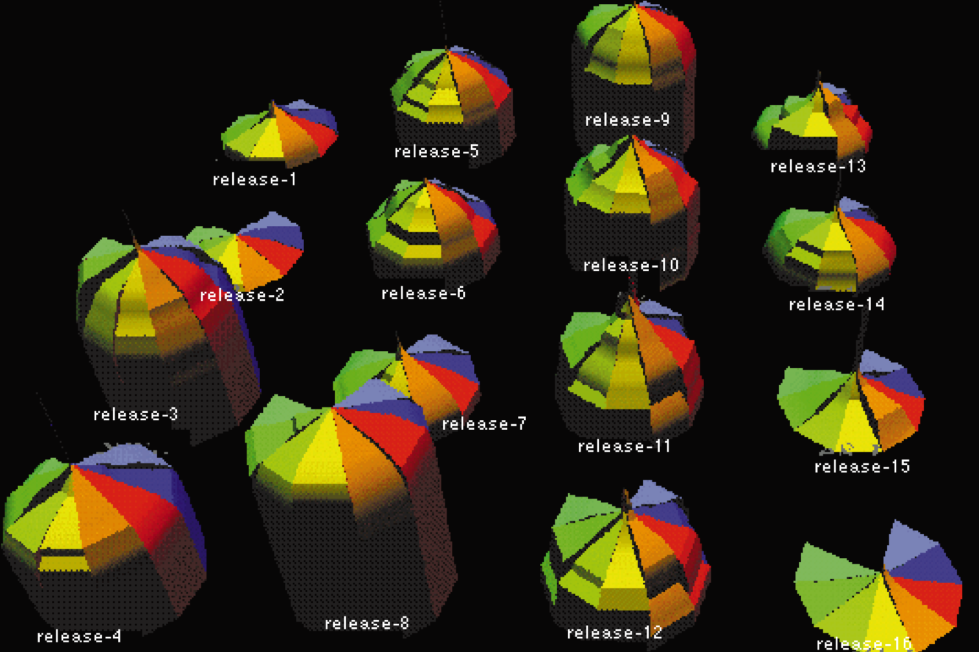
\includegraphics[width=\linewidth]{Chuan2.png}
  \caption{3D wheel}
   \label{fig:Chuan2}
\endminipage\hfill
\minipage{0.32\textwidth}
\centering
  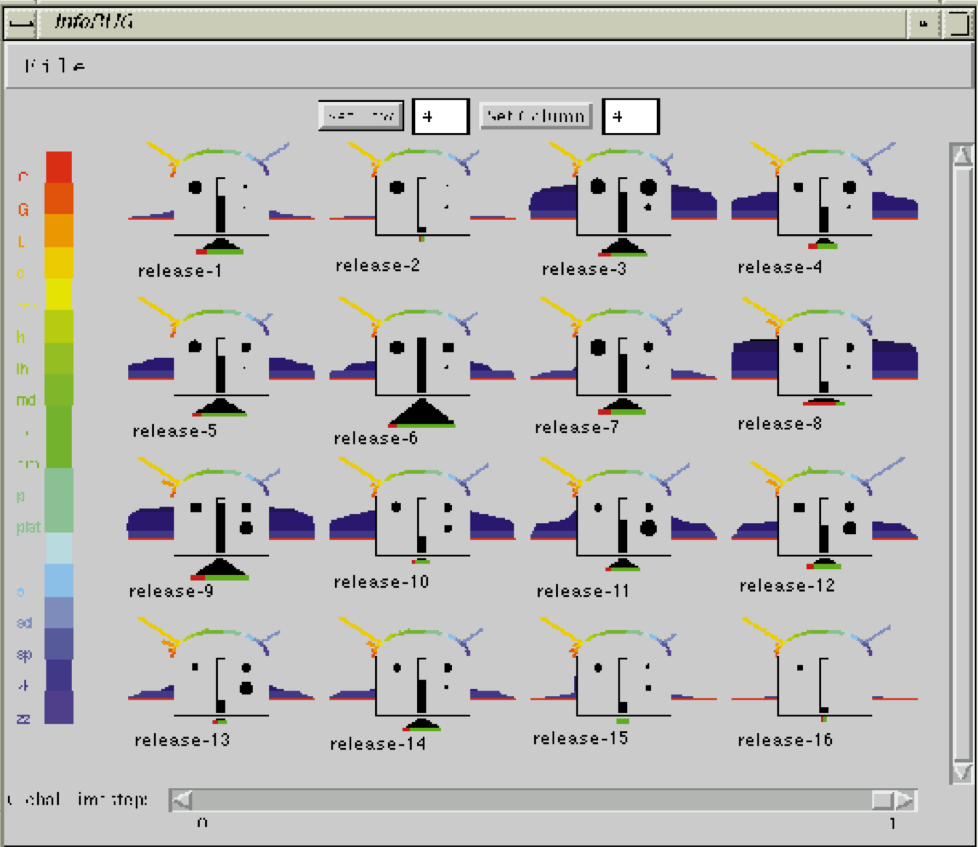
\includegraphics[width=\linewidth]{Chuan3.png}
  \caption{Infobug}
   \label{fig:Infobug}
\endminipage
\end{figure}
 
Also in 1998, Young and Munro \cite{Young1998} explored representations of software for program comprehension in VR. 

Finally, in 1999, Jacobson et al. \cite{Jacobson1999} introduced what we now know as de facto the standard language to visualize the design of a system: UML. 


% Edward Tufte has influenced the entire field of information visualization, including software visualization.
% 	[Tuf90] Edward Tufte. Envisioning Information. Graphics Press, 1990.
% 	[Tuf97] Edward Tufte. Visual Explanations. Graphics Press, 1997.
% 	[Tuf01] Edward Tufte. The Visual Display of Quantitative Information. Graphics Press, 2nd edition, 2001.

% \subsection{Software evolution visualization}
%https://www.inf.usi.ch/faculty/lanza/Downloads/Gall2006a.pdf
At the beginning of the 21st century, thanks to the spread of version control systems and the open-source movement, 
visualizing a software system's evolution became a more feasible activity thanks to publicly accessible system information.
As a result, many researchers focused their work on software evolution visualization.

Lanza \cite{Lanza2001} introduced the concept of the Evolution Matrix (\autoref{fig:EvolutionMatrix1}). 
It was a way to visualize the evolution of software without dealing with a large amount of complex data. 
Furthermore, this approach was agnostic to any particular programming language. 
The Evolution Matrix aimed to display the evolution of classes in object-oriented software systems. 
Each column represented a version of the system, and each row represented a different version of the same class.
Cells were filled with boxes whose size depended on evolutionary measurements. 
The evolution matrix allows us to make statements on the evolution of an object-oriented system at both the system and class levels. For example, in \autoref{fig:EvolutionMatrix2}, at system level, we are able to recover information regarding the size of the system, the addition and removal of classes, and the growth or stagnation phases in the evolution. 


\begin{figure}[ht]
\minipage{0.49\textwidth}
\centering
  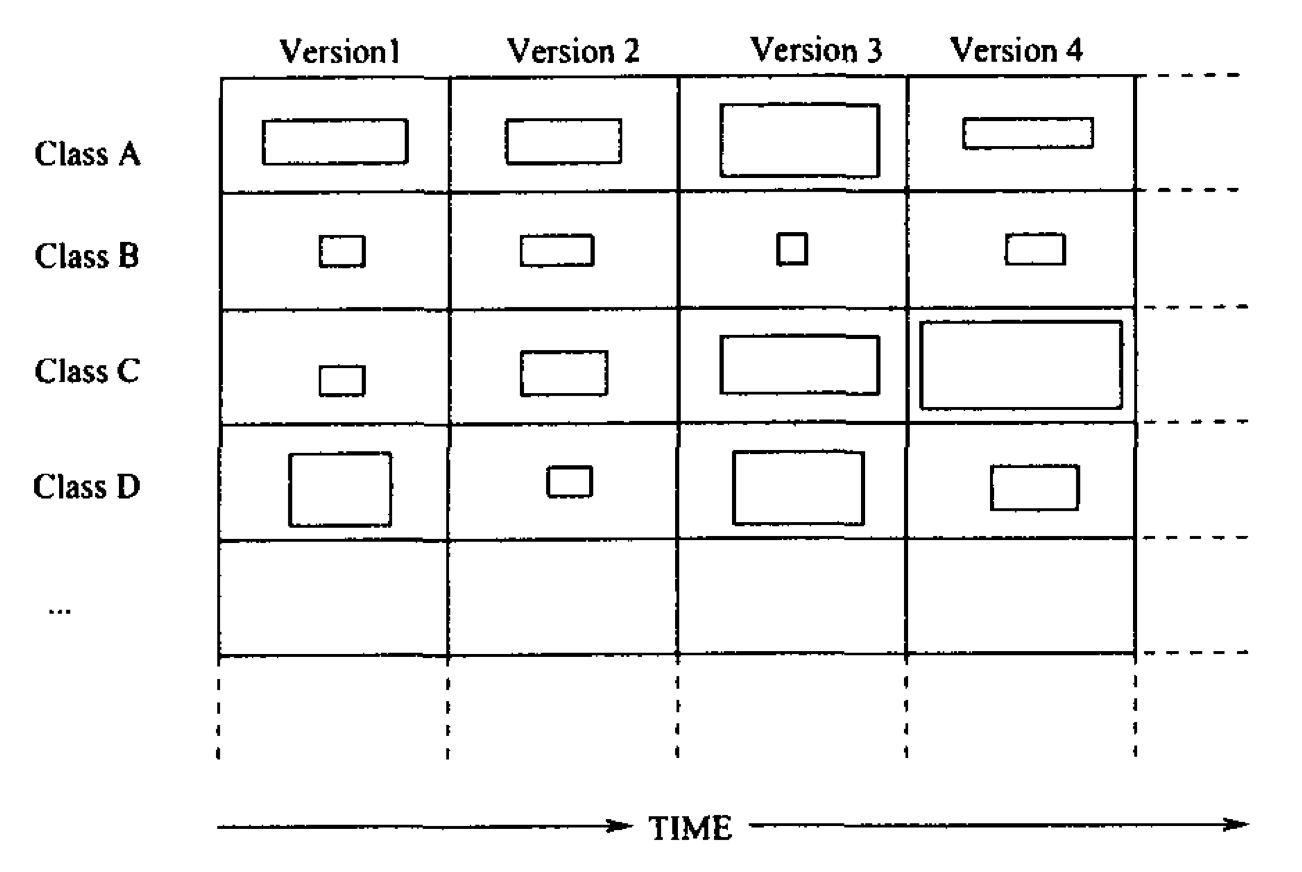
\includegraphics[width=\linewidth]{EvolutionMatrix1.png}
  \caption{A schematic display of the Evolution Matrix}
  \label{fig:EvolutionMatrix1}
\endminipage\hfill
\minipage{0.49\textwidth}
\centering
  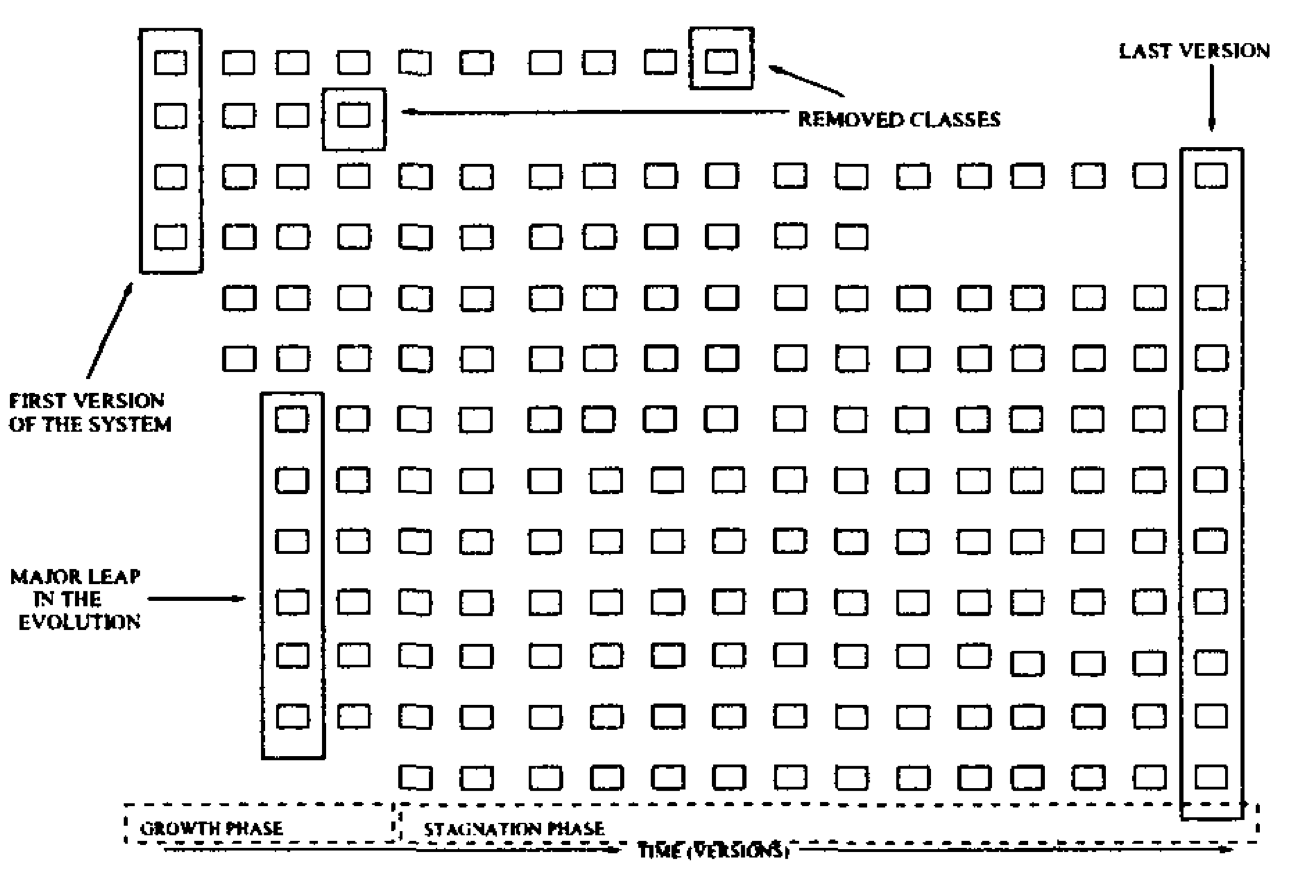
\includegraphics[width=\linewidth]{EvolutionMatrix2.png}
  \caption{Some characteristics of the Evolution Matrix}
  \label{fig:EvolutionMatrix2}
\endminipage\hfill
\end{figure}

Taylor and Munro \cite{Taylor2002} demonstrated that it was possible to use the data contained in a version control repository to visualize the evolution of a system.
They developed Revision Tower, a tool that showed change information at the file level. 
Pinzger et al. \cite{Pinzger2005} visualized the evolution of a software system through Kivat diagrams.
RelVis, the tool they developed, depicted a multivariate visualization (\autoref{fig:RelVis}) of the evolution of a system. It was built on Kiviat diagrams, designed to visualize multivariate data such as source code and evolution metrics. 
During the same year, Ratzinger et al. presented EvoLens \cite{Ratzinger2005}, a visualization approach and tool to 
explore evolutionary data through structural and temporal views.
Langelier et al. \cite{Langelier2005} investigated the interpretation of a city metaphor 
\cite{Knight2000} to add a new level of knowledge to the visual analysis.
D’Ambros and Lanza \cite{DAmbros2006} introduced the Discrete-Time Figure concept (\autoref{fig:TDT}). It was a visualization technique that embedded historical and structural data in a simple figure. 
Their approach depicted relationships between the histories of a system and bugs. 
They presented Evolution Radar \cite{DAmbros2006a} (\autoref{fig:Evoradar}), a novel approach to visualizing module-level and file-level logical coupling information.

\begin{figure}[H]
  \minipage{0.33\textwidth}
  \centering
    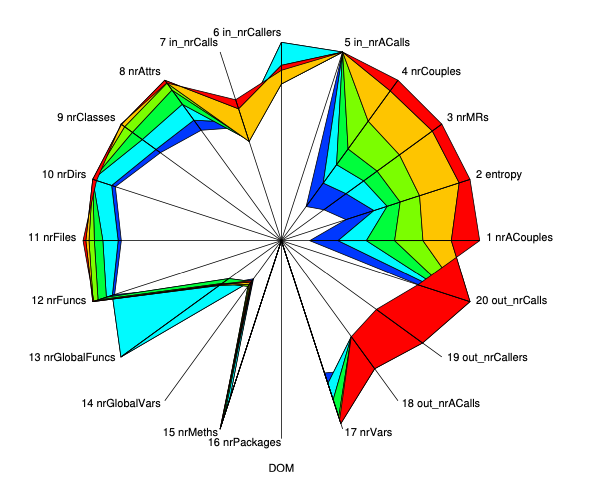
\includegraphics[width=\linewidth]{Pinzger2005_RelVis.png}
    \caption{RelVis}
      \label{fig:RelVis}
  \endminipage\hfill
  \minipage{0.33\textwidth}
  \centering
    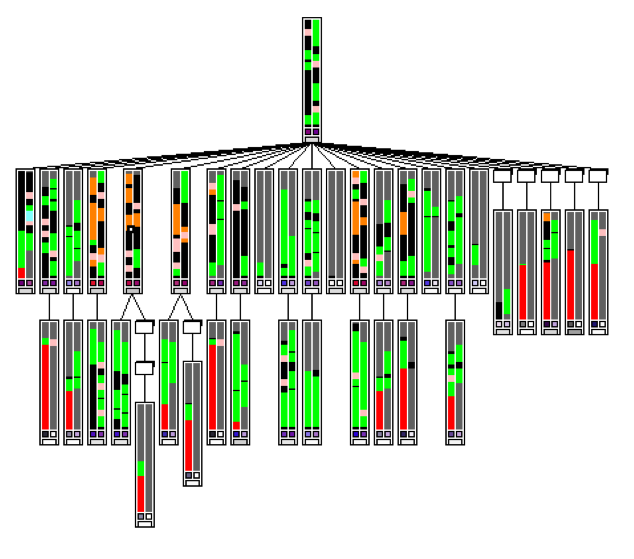
\includegraphics[width=\linewidth]{DAmbros2006.png}
    \caption{Tree of Discrete Time Figures}
    \label{fig:TDT}
  \endminipage\hfill
  \minipage{0.33\textwidth}
  \centering
  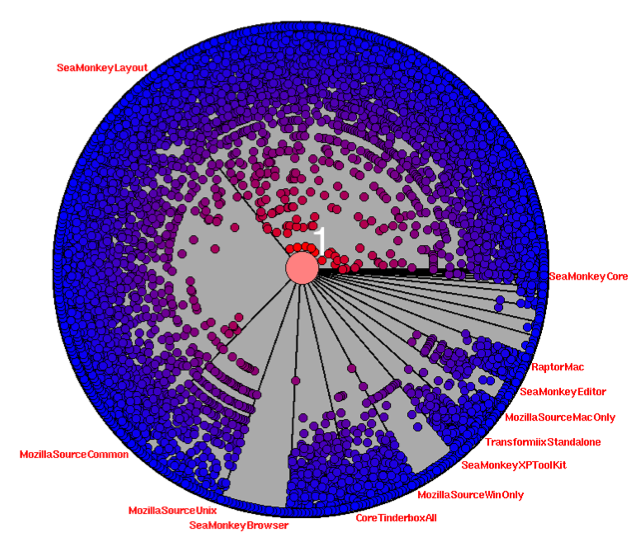
\includegraphics[width=\linewidth]{DAmbros2006a_EvoRadar.png}
  \caption{Evolution Radar}
  \label{fig:Evoradar}
\endminipage\hfill
  \end{figure}
  
Steinbrückner and Lewerentz \cite{Steinbrueckner2010} described a three-staged visualization approach to visualize large software systems. 
Their visualization was supported by a tool called Evo-Streets. 
Each stage of their approach yields a specific model that evolved through the stages. In the first stage, they created a model containing all the structure of a software system and its evolution. In the second stage, geometrics information is added, such as the city layout or landscape elevation. Finally, in the third stage, they added projections, colors, and symbols to the visualization. 

\begin{figure}[ht]
\centering
  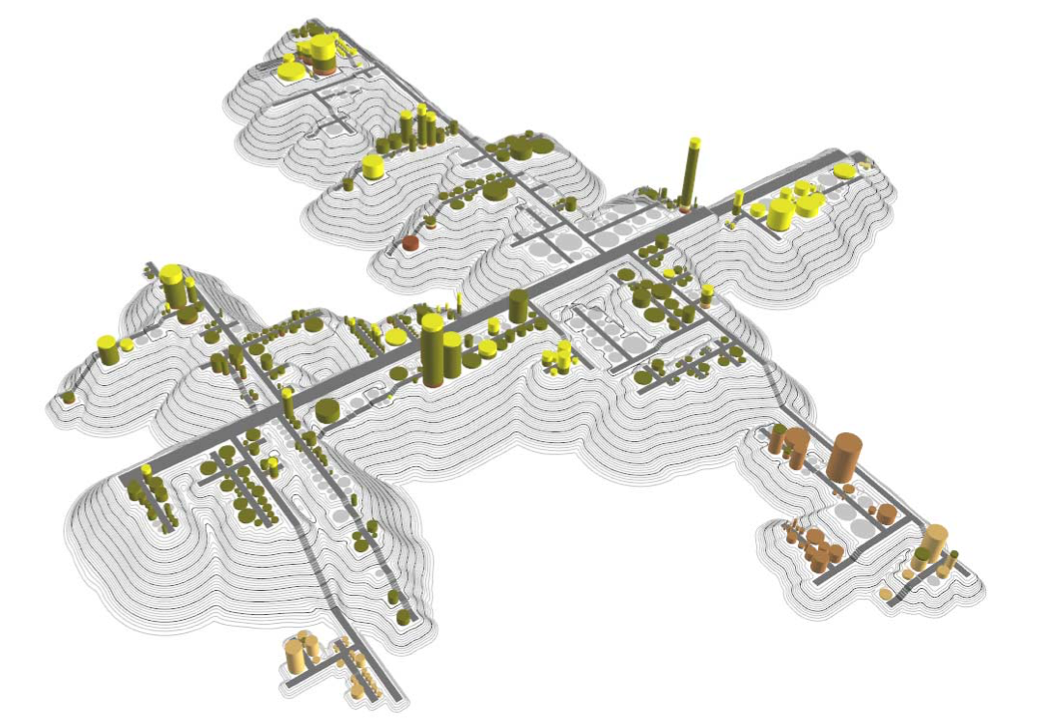
\includegraphics[width=0.9\linewidth]{Steinbrueckner2010.png} 
  \caption{Evo-Streets}
\end{figure}
 
Wettel revised the city metaphor to represent metrics meaningfully  \cite{Wettel2011}. 
In his thesis, he represented packages as districts and classes as buildings.
The metaphor was used for various purposes, e.g., reverse engineering, program comprehension, software evolution, or software quality analysis. 
He claimed that the city metaphor brought visual and layout limitations; for example, not all visualization techniques fit well.
Under those circumstances, he preferred simplicity over accuracy,
so he obtained a simple visual language that facilitated data comprehension. His approach was implemented as a software visualization tool 
called CodeCity (\autoref{fig:codecity}). 


\begin{figure}[ht]
\centering
  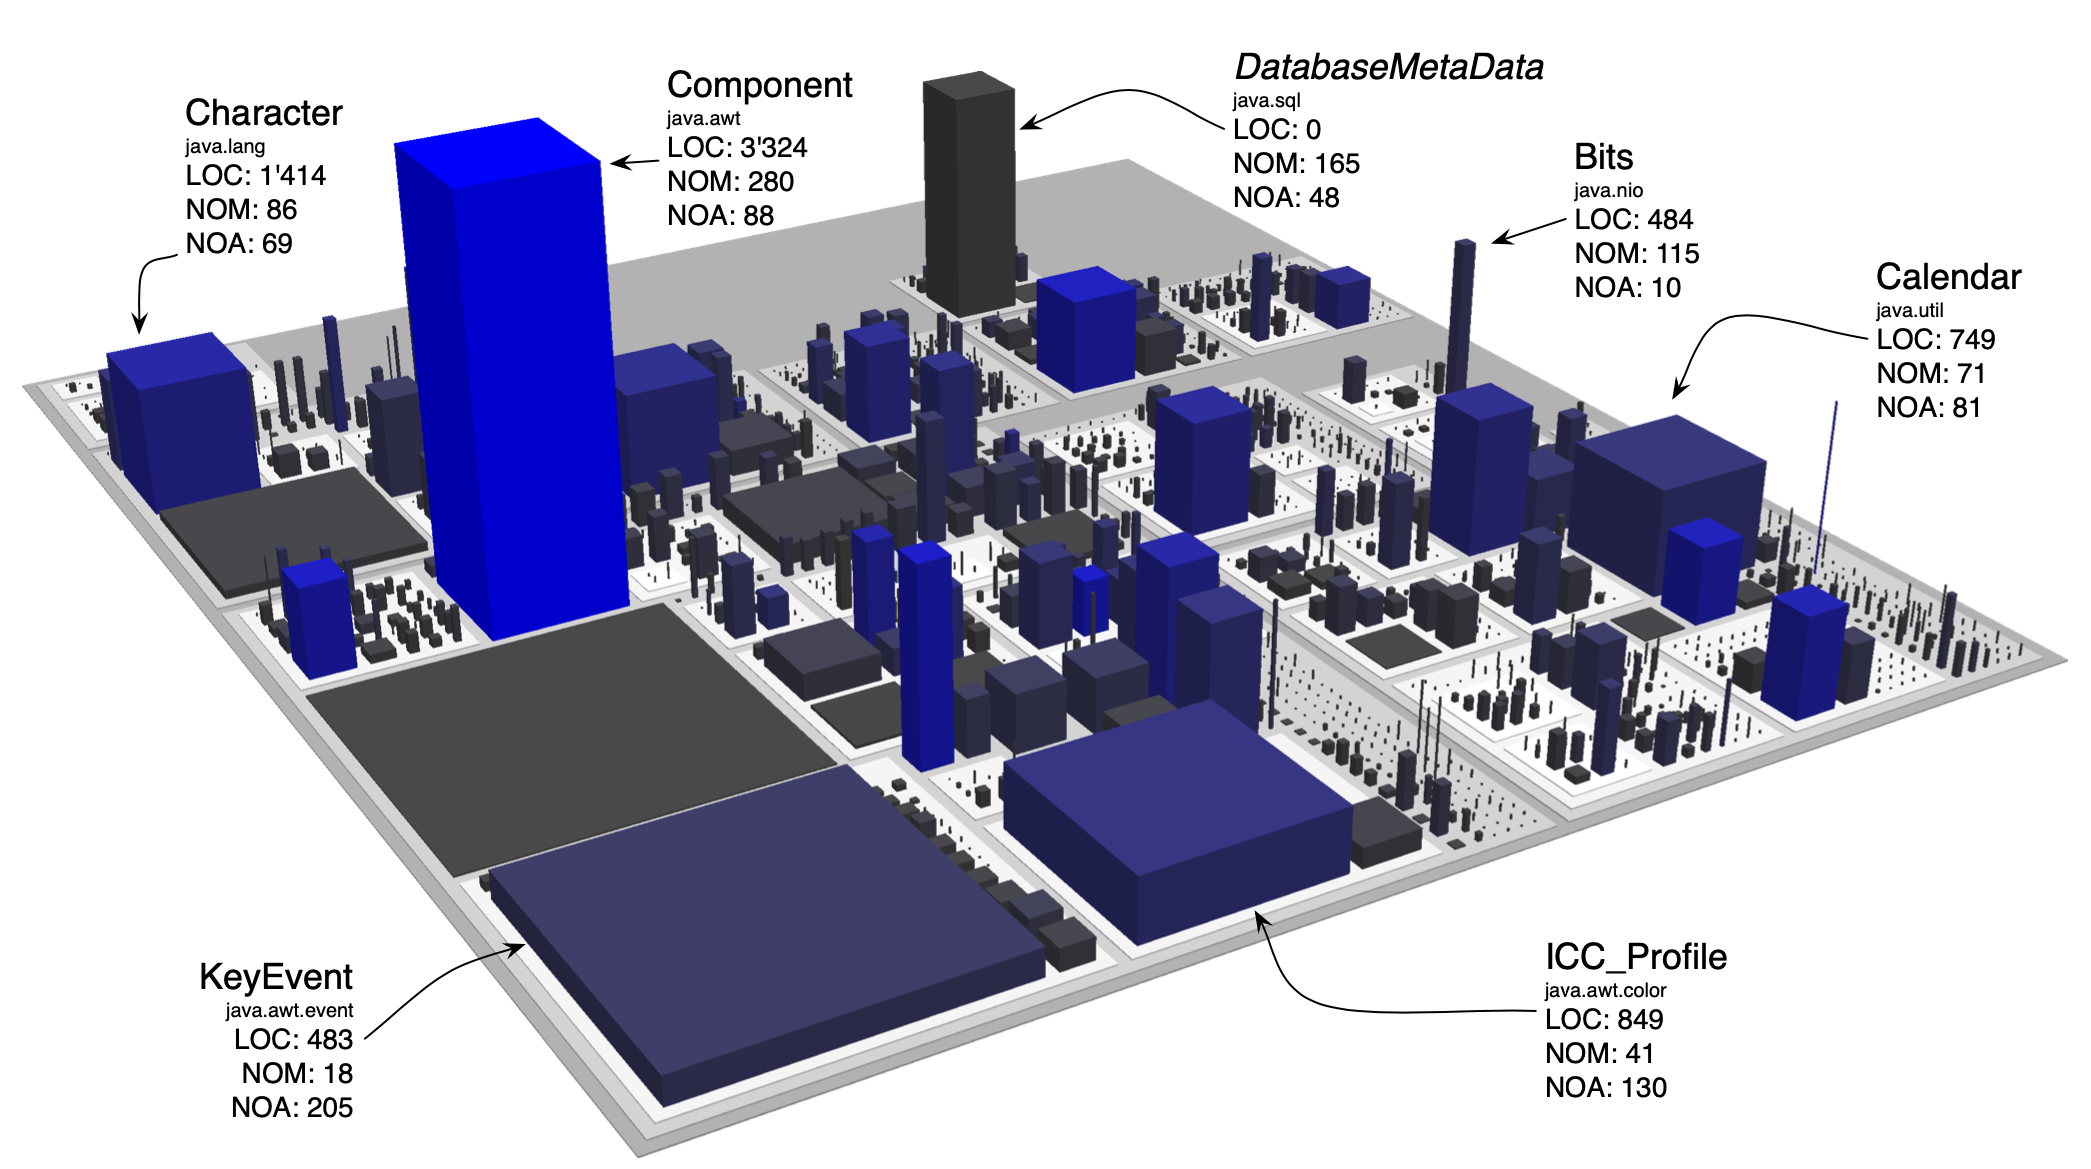
\includegraphics[width=0.9\linewidth]{CodeCity.png} 
  \caption{CodeCity}
  \label{fig:codecity}
\end{figure}

% ChronoTwigger 2014 https://ieeexplore.ieee.org/abstract/document/6980223
Ens et al. \cite{Ens2014} applied visual analytics methods to software repositories (\autoref{fig:ChronoTwigger}).
His approach helped users comprehend co-evolution information by visualizing how source and test files were developed together. 
% NN 2015 https://ieeexplore.ieee.org/document/7329727
Kapec et al. \cite{Kapec2015} proposed a graph analysis approach with augmented reality. 
They made a prototype of a tool that provided a graph-based visualization of software, and then they studied some interaction methods to control it with augmented reality.
% CuboidMatrix 2016 https://ieeexplore.ieee.org/document/7780168
Schneider et al. \cite{Schneider2016} presented a tool, CuboidMatrix (\autoref{fig:CuboidMatrix}), that employed a space-time cube metaphor to visualize a software system. 
A space-time cube is a well-known 3D representation of an evolving dynamic graph. 
% CityVR 2017 https://ieeexplore.ieee.org/abstract/document/8094470
Merino et al. \cite{Merino2017} aimed to augment software visualization with gamification. 
They introduced CityVR (\autoref{fig:CityVR}), a tool that displays a software system through the city metaphor with a 3D environment. 
Working with virtual reality, they scaled the city visualization to the physically available space in the room. 
Therefore, developers needed to walk to navigate the system. 

\begin{figure}[ht]
  \minipage{0.32\textwidth}
  \centering
    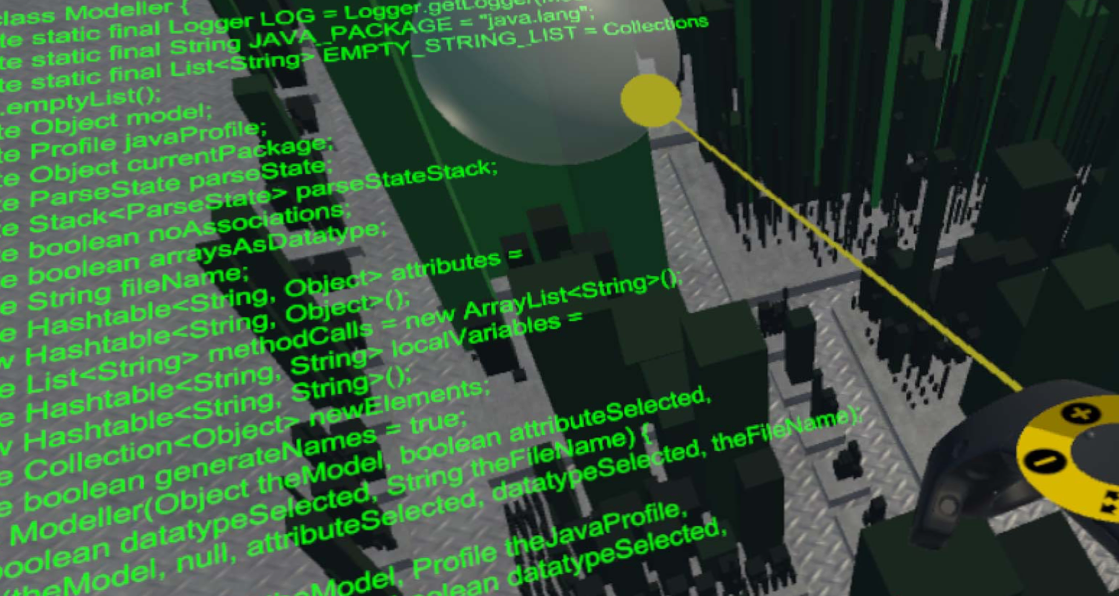
\includegraphics[width=\linewidth]{CityVR.png}
    \caption{CityVR}
    \label{fig:CityVR}
  \endminipage\hfill
  \minipage{0.32\textwidth}
  \centering
    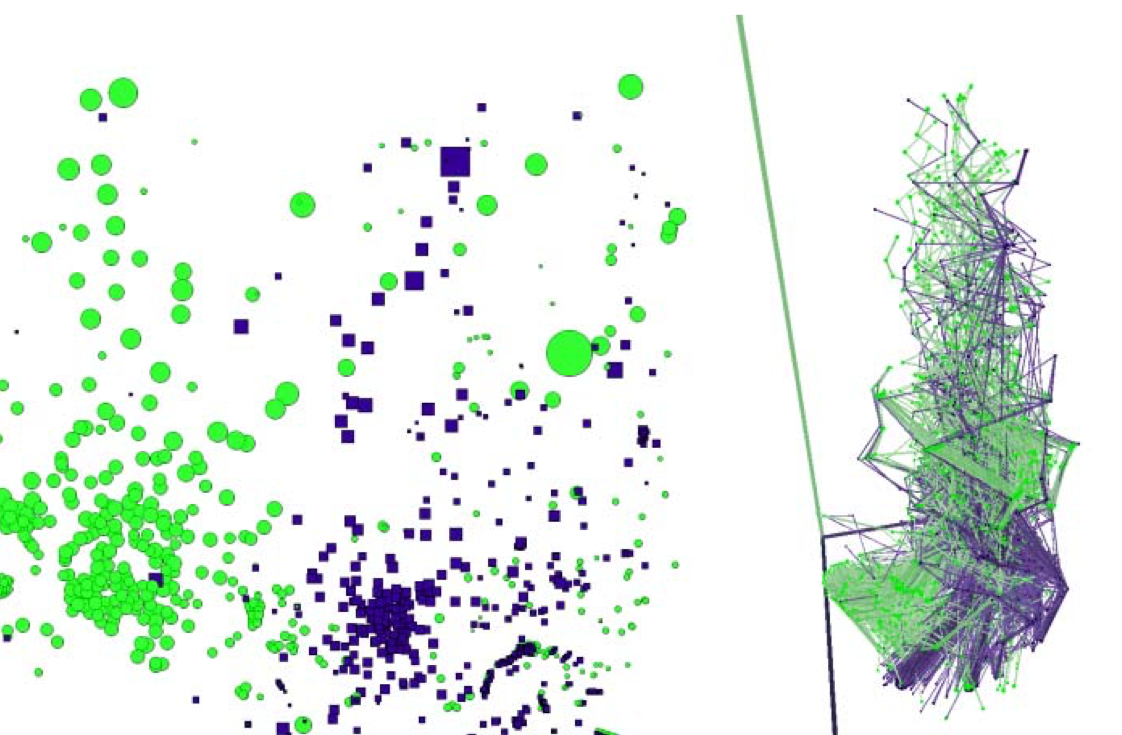
\includegraphics[width=\linewidth]{ChronoTwigger.png}
    \caption{ChronoTwigger}
    \label{fig:ChronoTwigger}
  \endminipage\hfill
  \minipage{0.32\textwidth}
  \centering
    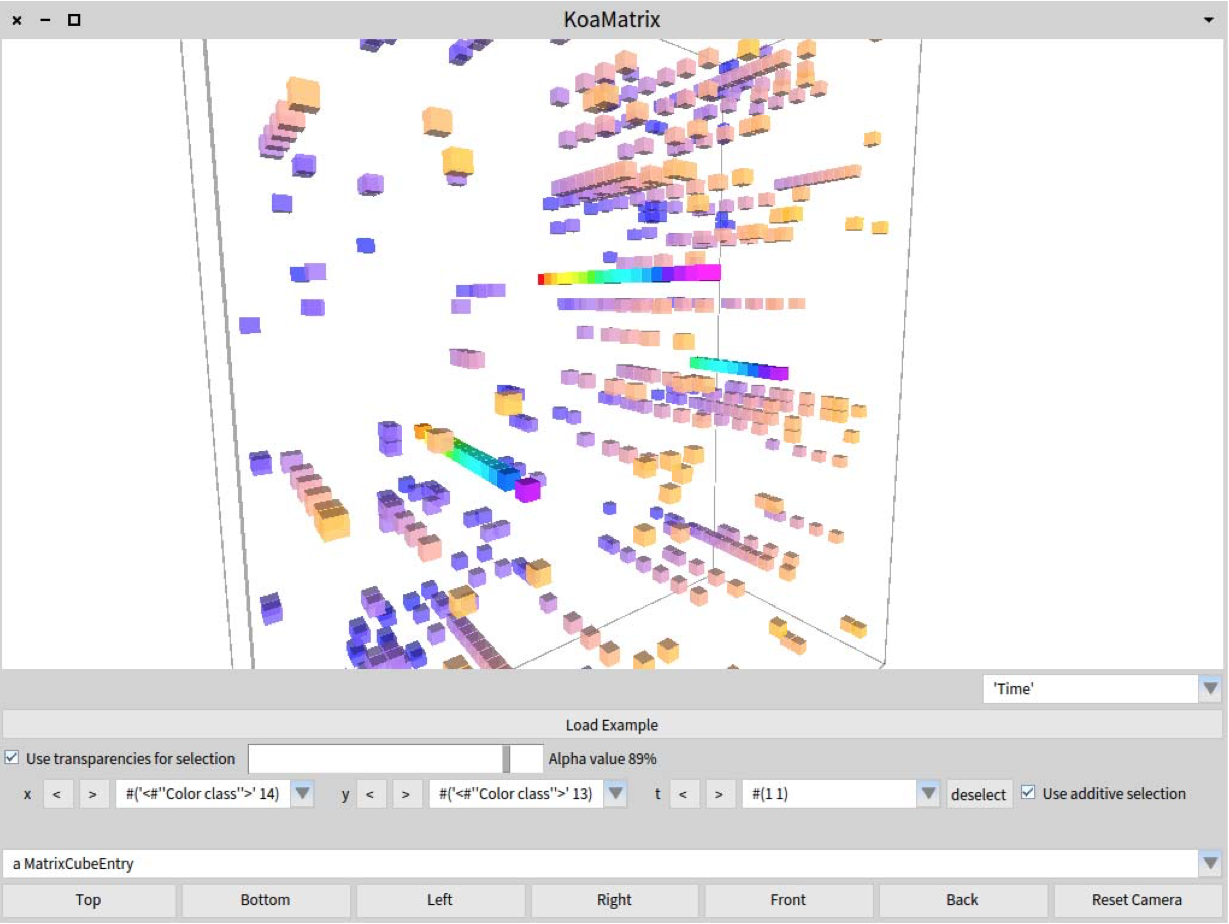
\includegraphics[width=\linewidth]{CuboidMatrix.png}
    \caption{CuboidMatrix}
    \label{fig:CuboidMatrix}
  \endminipage
  \end{figure}
  

% Code Park 2017 https://ieeexplore.ieee.org/abstract/document/8091185
Khaloo et al. \cite{Khaloo2017} revised the idea of gamification with a 3D park-like environment. They mapped each class in the codebase with a facility. The wall structure depended on the class' constituent parts, e.g., methods and signatures. 
% Evo-Clocks 2019 https://ieeexplore.ieee.org/document/8900965
Finally, we mention Alexandru et al., who proposed a method to visualize software structure and evolution 
with reduced accuracy and a fine-grained highlighting of changes in individual components \cite{Alexandru2019}. \autoref{fig:EvoClock} shows a view of Evo-Clocks, the tool they developed. 

\begin{figure}[ht]
\centering
  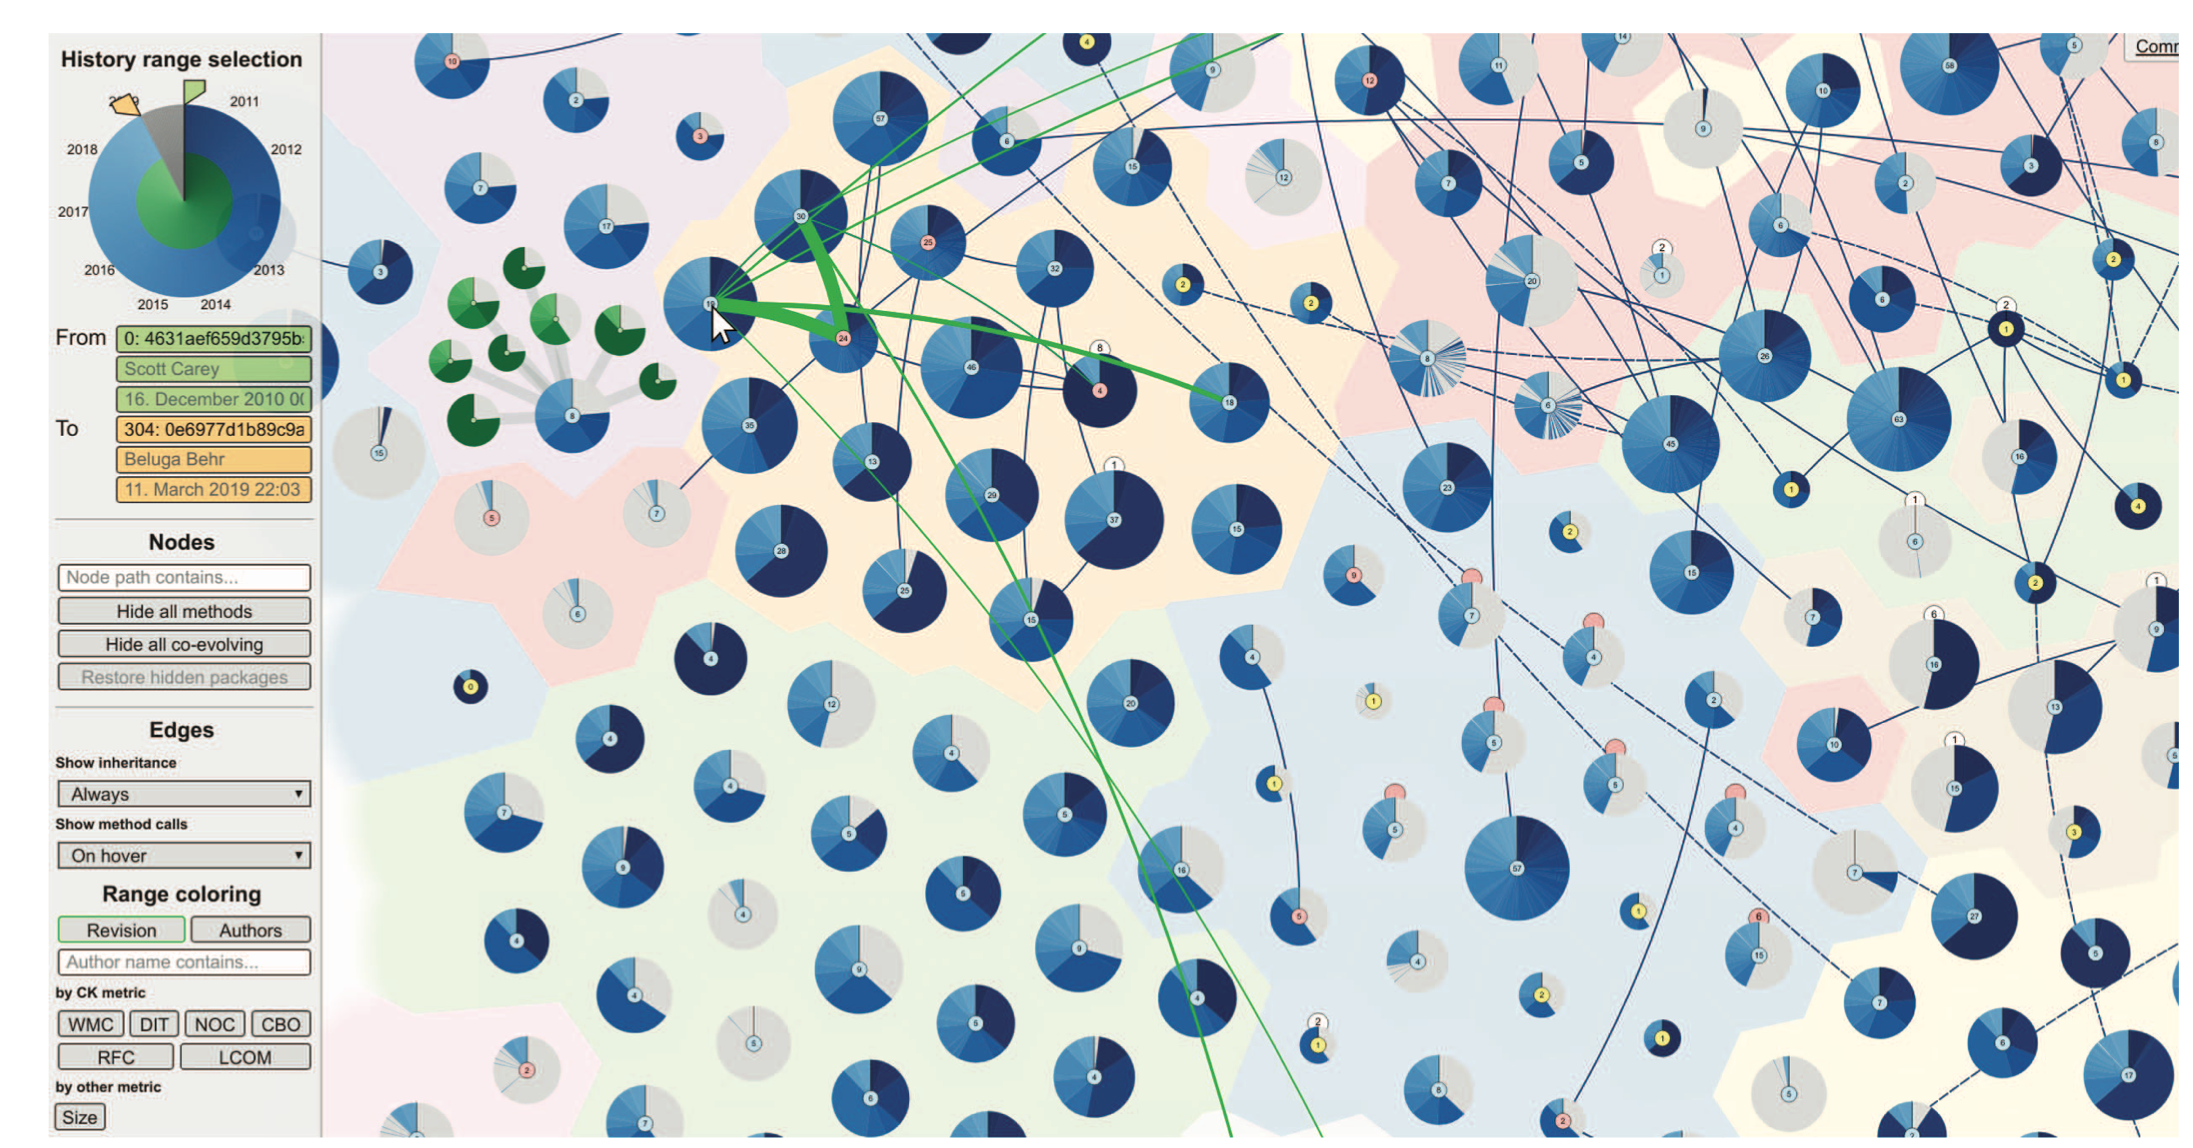
\includegraphics[width=0.9\linewidth]{Alexandru_EvoClock.png} 
  \caption{Evo-Clocks}
      \label{fig:EvoClock}

\end{figure}


\section{Software Evolution Analysis}

Version control systems track historical data in repositories about the evolution of a system. Git has become the most popular version control system today since Linus Torvald introduced it in 2005. Many collaboration platforms (e.g., GitHub and GitLab) also rely on it. With the increased popularity of such platforms, millions of open-source systems are developed publicly. They have also become popular targets for Mining Software Repositories (MSR) research.

D'Ambros et al. \cite{SoftwareEvolution} presented an analysis and visualization techniques to understand software evolution. 
They developed an approach based on a Release History Database (RHDB). 
It is a database that stores historical information about source code and bugs. 
The strength of RHDB (\autoref{fig:RHDB}) was the association between historical versions of flies and bugs. 
Having this information stored in a database, they were able to run an evolution analysis to obtain information such as the number of developers needed to fix a bug.   

Finally, they concluded two main challenges in MSR:
\begin{itemize}
  \item Technical challenge: repositories contain a sheer amount of data, posing scalability problems. 
  \item Conceptual challenge: how to leverage the collected data. 
  Most of the approaches to visualizing software evolution have unanswered questions about the effectiveness of the comprehension. 
\end{itemize}

\begin{figure}[H]
\centering
  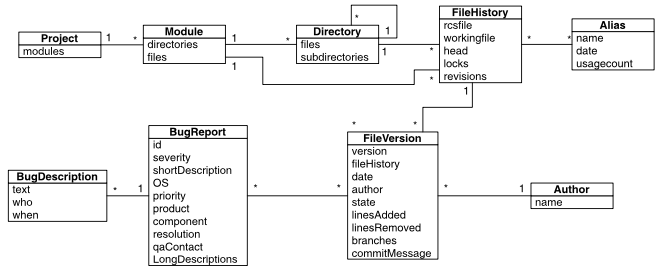
\includegraphics[width=0.9\linewidth]{RHDB.png} 
  \caption{RHDB}
  \label{fig:RHDB}
\end{figure}
 


% The promises and perils of mining GitHub  https://dl.acm.org/doi/abs/10.1145/2597073.2597074
In 2022, there are around 200 million GitHub repositories.\footnote{https://en.wikipedia.org/wiki/GitHub}
Even if it seems a promising data source, Kalliamvakou et al. raised some issues with its mining \cite{Kalliamvakou2014}.
For example, they found that a repository does not always match a project. 
A reason for this can be that most repositories had very few commits before becoming inactive.
Over 70\% of the GitHub projects were personal when they did their research, and some weren't used for software development. 
Finally, the last perils they raised were related to GitHub features improperly used by developers.
They considered only projects with a good balance between the number of commits, 
the number of pull requests, and the number of contributors to find actively developed repositories. 
 

% PyDriller https://dl.acm.org/doi/abs/10.1145/3236024.3264598
Spadini, Aniche, and Bacchelli \cite{Spadini2018} developed a Python framework called PyDriller, enabling users to mine software repositories. 
Their tool can be used to extract information about the evolution of a software system from a git repository.  

We also mention the work of Salis and Spinellis \cite{Salis2019}.
They introduced RepoFS, a tool that allows navigating a git repository as a file system. 
Their approach sees commits, branches, and tags as a separate directory tree. 
\autoref{fig:RepoFS} shows an example of a repository data structure. 

\begin{figure}[H]
\centering
  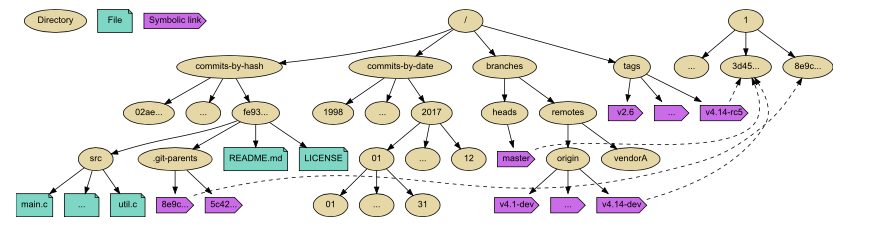
\includegraphics[width=0.9\linewidth]{Salis2019.png} 
  \caption{RepoFS}
  \label{fig:RepoFS}
\end{figure}

Clem and Thomson \cite{Clem2021}, members of the semantic code team at GitHub, built a static analyzer of repositories to implement symbolic code navigation. 
That feature was released on GitHub in 2020 years ago and lets developers click on a name identifier to navigate to the definition of the selected entity. 
They were looking for a solution without scalability problems. 
Moreover, they built the symbolic navigation feature around the following ideas:
\begin{itemize}
  \item Zero configuration needed by the owner of a repository.
  \item Incrementality of the process. There was no need to process the entire repository for every commit made by a developer. Instead, they analyzed only the files changed. 
  \item Language agnosticism of the static analysis. 
\end{itemize}

Working on that feature, they recognized the difficulty of scaling a static analysis to large and rapidly changing codebases.
Nevertheless, their idea was to have an agnostic static analyzer, but they could not reach this goal, and they were forced to implement it for nine programming languages.  

\section{Program Auralization}
\begin{figure}[ht]
\centering
  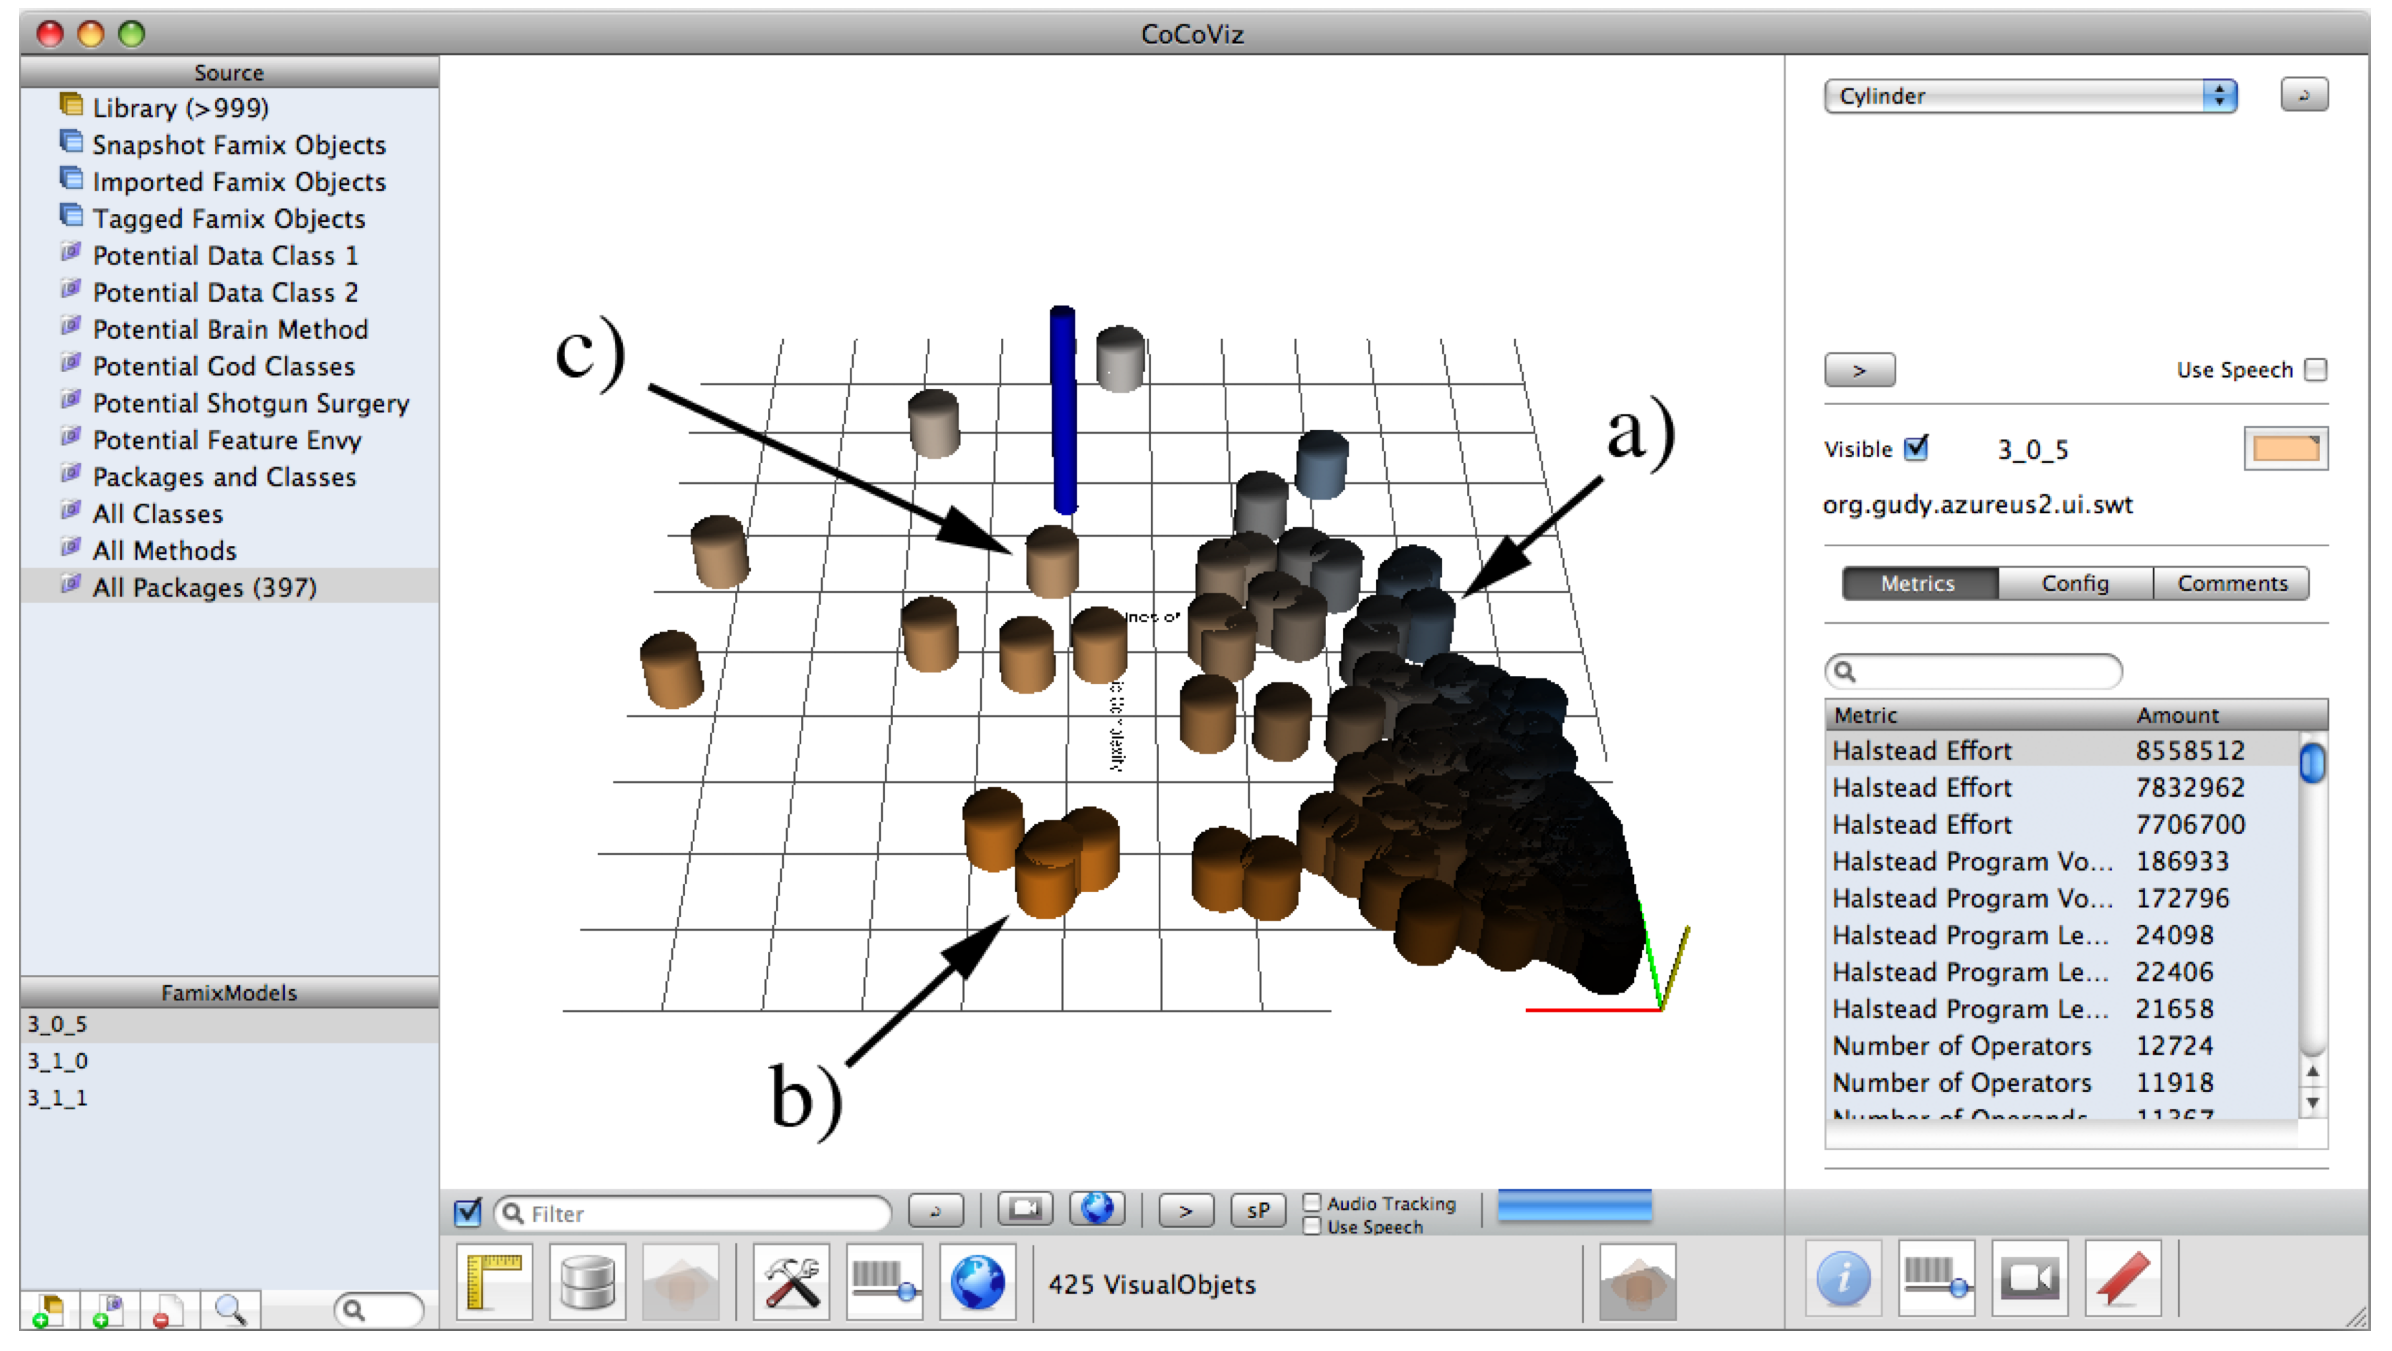
\includegraphics[width=0.9\linewidth]{CocoViz.png} 
  \caption{CocoViz}
  \label{fig:cocoviz}
\end{figure}


External auditory representations of programs (known as \quotes{program auralization}) is a research field getting even more interest in recent years.

% InfoSound https://ieeexplore.ieee.org/document/205229
Sonnenwald et al. made one of the first attempts \cite{Sonnenwald1990}.
They tried to enhance the comprehension of complex applications by playing music and special sound effects. 
This approach was supported by a tool called InfoSound.
It was mainly adopted to understand the program's behavior. 

Many other researchers followed this first technique. To cite some of them, DiGiano and Baecker \cite{DiGiano1993} made LogoMedia, a tool to associate non-speech
 audio with program events while the code is being developed. 
Jameson \cite{Jameson1994} developed Sonnet audio-enhanced monitoring and debugging tool.  
Alty and Vickers \cite{Vickers2003} had a similar idea. Using a structured musical framework, they could map the execution behavior of a program to locate and diagnose software errors. 
 
% EXTERNAL AUDITORY REPRESENTATIONS OF PROGRAMS https://smartech.gatech.edu/bitstream/handle/1853/50854/Vickers2004a.pdf?sequence=1&
Despite the usefulness of these tools, they adopted an essential kind of mapping, and thus they had a limited musical representation. 
Vickerts \cite{Vickers2004} found the necessity of a multi-threaded environment to enhance the comprehension given by the musical representation. 
He proposed adopting an orchestral model of families of timbres to enable programmers to distinguish between different activities of different threads.

%The size and the complexity of systems can represent a problem for the effectiveness of a visual representation of a software system.
%Having a large number of visual information, observers might find it difficult to focus only on the relevant aspects. 
% CocoViz https://ieeexplore.ieee.org/document/5070558
Boccuzzo and Gall \cite{Boccuzzo2009} supported software visualization with sonification, the use of non-speech audio to convey information or perceptualize data. 
They used audio melodies to improve navigation and comprehension of their tool, called CocoViz (\autoref{fig:cocoviz}).
Their ambient audio software exploration approach exploited audio to describe an entity's position in space intuitively. 
Thanks to the adoption of surround sound techniques, the observers perceived the origin of an audio source so it could adjust their navigation in the visualization.
Each kind of entity played a different sound based on mapping criteria.



 
% Orchestrating change: An artistic representation of software evolution https://ieeexplore.ieee.org/document/6747192 
McIntosh et al. \cite{McIntosh2014} explored the use of parameter-based sonification to produce a musical interpretation of the evolution of a software system.
Their technique mapped musical rests to an inactive period of development, consonance, and dissonance to interesting phenomena (like co-changing components).
% Software Musification https://ieeexplore.ieee.org/document/8107958
Finally, Mancino and Scanniello \cite{Mancino2017} presented an approach to transforming source code metrics into a musical score that can be both visualized and played. 


\section{Conclusion}

We have seen many different techniques and tools focused on visualizing the source code of software systems, their evolution, or their metrics.
Our evolution focuses on the evolution of a software system and how its metrics change over its history. 
In contrast to what some tools did, we do not focus on the evolution of code bugs.

The codebase of a system is composed of a group of files. In our approach, each file represents a system entity that mutates over time.
It is not based on a previously identified metaphor, such as CodeCity or CityVR with the city metaphor.
We created a new layout where the position of each entity is defined by its discovery time. 

At present, git has become the standard tool for version control. 
Having this in mind, we aim to find a suitable model to represent the histories of mined git repositories.
Therefore, we created a model inspired by the EvolutionMatrix, but with adjustments to make it work with git.

As Clem and Thomson \cite{Clem2021} team did, we propose a scalable approach that works with large repositories. 
It differs from what they did because we are not focused on a semantic analysis of the source code; instead, we extract source code metrics. 
Moreover, our technique is purely language-agnostic.

Finally, we extended our approach with an auralization approach to compose music based on a system’s evolution. 
Conversely to state-of-the-art tools, we used a multithreaded environment to play the musical notes. 
Whereas CocoViz used audio melodies to support the navigation of space created for the visualization, we mapped sounds to the magnitudes of changes in a given moment. 





